\documentclass[tikz,border=1pt]{standalone}
\usepackage{fontspec}
\setmainfont{Times New Roman}

\usetikzlibrary{positioning,arrows.meta}

% Pure black-and-white palette for print
\begin{document}
\hyphenpenalty=10000
\exhyphenpenalty=10000
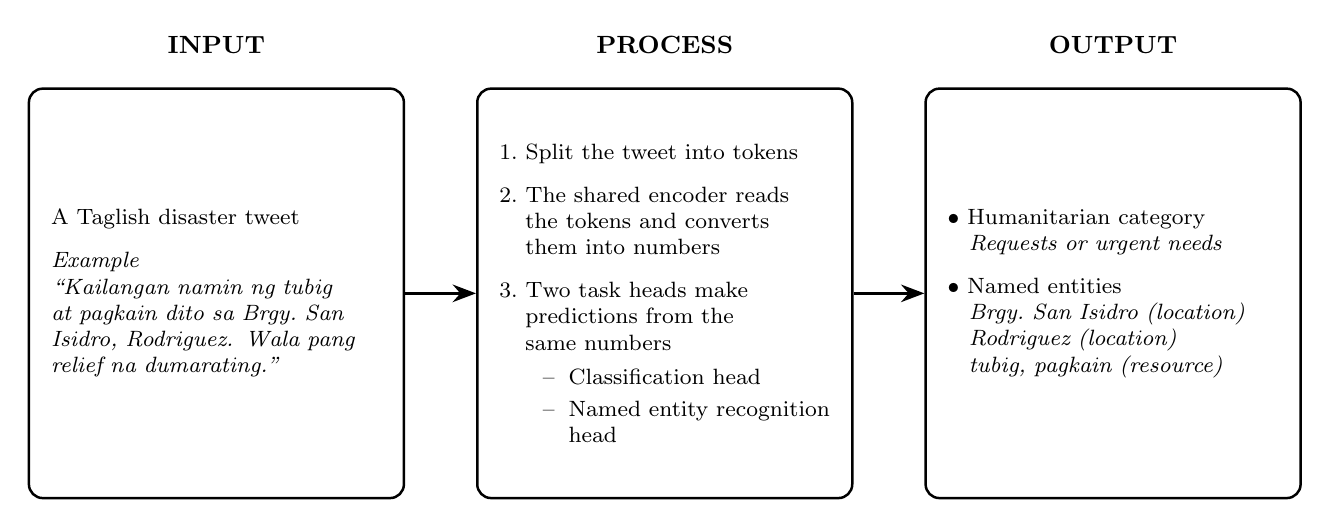
\begin{tikzpicture}[
    font=\small,
    >=Stealth,
    iobox/.style={draw=black, rounded corners=5pt, align=left,
        text width=4.2cm, minimum height=5.2cm, inner sep=8pt,
        font=\footnotesize, line width=0.9pt},
    head/.style={font=\small\bfseries},
    bigarrow/.style={->, very thick}
]

    \node[iobox] (input) {
        A Taglish disaster tweet\\[6pt]
        \textit{Example}\\
        \textit{``Kailangan namin ng tubig at pagkain dito sa Brgy.\ San Isidro, Rodriguez. Wala pang relief na dumarating.''}
    };

    \node[iobox, right=0.9cm of input] (process) {
        1.~Split the tweet into tokens\\[6pt]
        2.~The shared encoder reads\\
        \hspace*{1.1em}the tokens and converts\\
        \hspace*{1.1em}them into numbers\\[6pt]
        3.~Two task heads make\\
        \hspace*{1.1em}predictions from the\\
        \hspace*{1.1em}same numbers
        \begin{itemize}
            \setlength{\itemsep}{0pt}
            \item[--] Classification head
            \item[--] Named entity recognition head
        \end{itemize}
    };

    \node[iobox, right=0.9cm of process] (output) {
        $\bullet$~Humanitarian category\\
        \hspace*{0.9em}\textit{Requests or urgent needs}\\[6pt]
        $\bullet$~Named entities\\
        \hspace*{0.9em}\textit{Brgy.\ San Isidro (location)}\\
        \hspace*{0.9em}\textit{Rodriguez (location)}\\
        \hspace*{0.9em}\textit{tubig, pagkain (resource)}
    };

    \node[head, above=0.3cm of input] {INPUT};
    \node[head, above=0.3cm of process] {PROCESS};
    \node[head, above=0.3cm of output] {OUTPUT};

    \draw[bigarrow] (input) -- (process);
    \draw[bigarrow] (process) -- (output);

\end{tikzpicture}
\end{document}
